\documentclass[a4paper,12pt]{article}
\usepackage[utf8]{ inputenc}
\usepackage[ngerman]{babel}
\usepackage[a4paper, left=2.5cm, right=2.5cm]{geometry}
\usepackage{graphicx}
\usepackage{subcaption}
\usepackage{fancyhdr}
\usepackage{pdfpages}
\usepackage{listings}
\usepackage{hyperref}
\usepackage[official]{eurosym}
\usepackage{float}

\pagestyle{fancy}
\lstset{
	language=Matlab,
	breaklines=true,
	morekeywords={matlab2tikz},
	keywordstyle=\color{blue},
	morekeywords=[2]{1}, keywordstyle=[2]{\color{black}},
	identifierstyle=\color{black},
	stringstyle=\color{mylilas},
	commentstyle=\color{mygreen},
	showstringspaces=false,
	mathescape=true
	emph=[1]{for,end,break},emphstyle=[1]\color{red},
}

\hypersetup{
	colorlinks=true,
	linkcolor=blue,
	filecolor=magenta,      
	urlcolor=cyan
}

\lhead{Standort von Windenergieanlagen}
\chead{}
\rhead{Gruppe D}

\begin{document}
	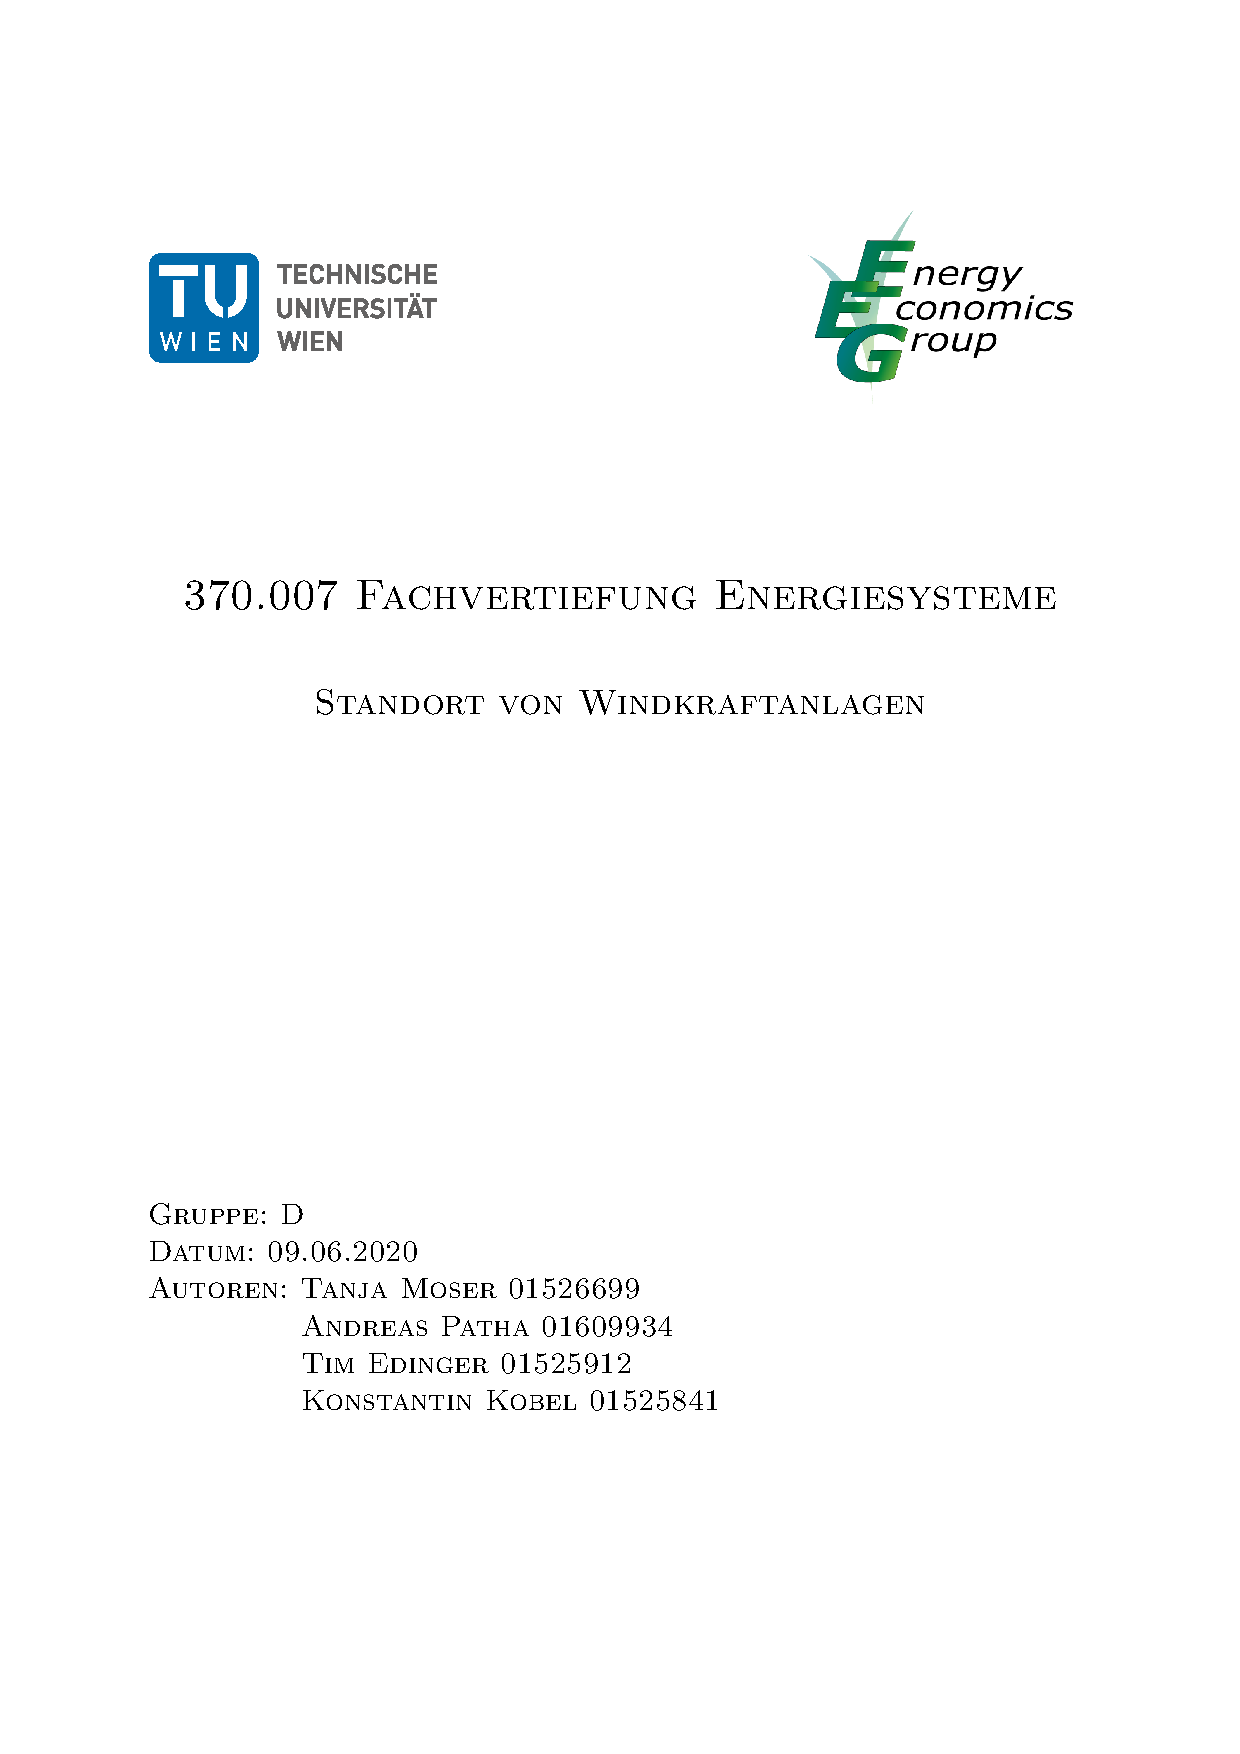
\includepdf{Protokoll_titlepage.pdf}

	\newpage
	\tableofcontents

	\newpage
	
	\section{Einleitung (Konzept)}
	Für die 5. Abgabe möchten wir unterschiedlichen Standorte von Windenergieanlagen miteinander vergleichen.\\ \par
	\noindent Im Speziellen sollen zwei Aspekte mit einander verglichen werden:
	\begin{itemize}
		\item Offshore vs. Onshore
		\item Standort in Europa (Äquatornähe vs. Polnähe)
	\end{itemize}
	In beiden Fällen wird von unterschiedlichen Höhen der Windenergieanlagen ausgegangen.\\ \par
	\noindent Der Vergleich erfolgt auf Basis folgender Punkte:
	\begin{itemize}
		\item Ertrag
		\item Betriebskosten und Investitionskosten
		\item Barwert
		\item Lebensdauer
	\end{itemize}
	Die relevanten Daten werden folgenden Quellen entnommen:
	\begin{itemize}
		\item Informationen zu den Betriebs- und Investitionskosten einer Onshore Windenergieanlage: \href{https://www.diplomarbeitsboerse.info/wp-content/uploads/%C3%96konomische-Bewertung-der-Windkraft_Bsp-Gro%C3%9Fhofen.pdf}{Ökonomische Bewertung der Windkraft}, 
		\href{https://elite.tugraz.at/Jungbauer/6.htm}{Wirtschaftlichkeit von Windenergieanlagen},  \href{http://windmonitor.iee.fraunhofer.de/windmonitor_de/3_Onshore/5_betriebsergebnisse/4_betriebskosten/}{Betriebskosten}
		\item Informationen zu den Betriebs- und Investitionskosten einer Offshore Windenergieanlage:
		\href{http://windmonitor.iee.fraunhofer.de/windmonitor_de/4_Offshore/5_betriebsergebnisse/4_Investitionskosten/}{Investitionskosten}
		\item Winddaten für das Jahr 2018, für Europa:
		\href{http://www.soda-pro.com/web-services/meteo-data/merra}{MERRA-2 meteorological re-analysis}
	\end{itemize}
	Ebenfalls wird auf die vom Institut zur Verfügung gestellten Daten (\href{http://www.sciencedirect.com/}{http://www.sciencedirect.com/}, \href{https://scholar.google.com/}{https://scholar.google.com/}, \href{http://catalogplus.tuwien.ac.at/}{http://catalogplus.tuwien.ac.at/}) zurückgegriffen.
	
	\newpage
	
	\section{Berechnungen}
	\subsection{Leistung und Ertrag}
	Wind stellt strömende Luftmassen dar. Da es sich um eine bewegte Masse handelt, kann die kinetische Energie dieser Masse berechnet werden.\newline
	Die Formel zur Berechnung der kinetischen Energie einer bewegten Masse $m$ mit einer Geschwindigkeit $v$ ist allgemein
	\begin{equation}
	E_{Wind} = \frac{1}{2}*m*v^2
	\end{equation}
	\noindent Ersetzt man die Masse durch das Produkt aus dem Volumen und der Dichte und leitet man die Formal nach der Zeit ab, erhält man
	\begin{equation}
	P_{Wind} = \frac{1}{2}*\rho_L*\dot{V_L}*v^2
	\end{equation}
	Das zeitabhängige Volumen kann nun durch das Produkt aus der Windgeschwindigkeit und der Querschnittsfläche ersetzt werden. Dadurch erhält man schlussendlich
	\begin{equation}
	P_{Wind} = \frac{1}{2}*\rho_L*A*v^3
	\end{equation}
	Zusätzlich zur Leistung des Windes muss der Leistungsbeiwert berücksichtig werden. Der Leistungsbeiwert gibt den Quotienten aus genutzter zu ankommender Windleistung $c_p = \frac{P}{P_0}$ an. Für Windenergieanlagen generell gilt, dass der Leistungsbeiwert maximal $0.5926$ betragen kann. Es ist also nur möglich knapp unter $60\%$ der Energie des Windes in elektrische Energie umzuwandeln (ohne Berücksichtigung des Wirkungsgrades des Getriebes und des Generators).\newline
	Die schlussendlich von einer Windenergieanlage produzierte Leistung errechnet sich aus folgender Formel:
	\begin{equation}
	P = P_{Wind}*c_p*\eta
	\end{equation}
	Mangels genauer Messwerte zum Leistungsbeiwert und dem Wirkungsgrad der Windenergieanlage, haben wir das Produkt aus beide aus den Nennwerten errechnet.\newline
	Daraus ergibt sich
	\begin{equation}
	c_p * \eta = \frac{P_N}{\frac{1}{2}\bar{\rho}*A*v_N^3}
	\end{equation}
	Für den Fall der Onshore Windenergieanlage entspricht das einem Faktor von $2.6156e-07$. Im Falle der Offshore Anlage beträgt dieser Faktor $2.6124e-07$.\\ \par
	Der Ertrag entspricht dem Integral über die Leistung. \newline Demnach gilt\begin{equation}
	E_A = \sum_{i} E_i = T * \sum_{i} h_i * P_{el, i}
	\end{equation}
	\subsection{Windgeschwindigkeit}
	Die für die folgenden Berechnungen notwendigen Winddaten werden aus dem Tool "MERRA 2" (Modern-Era Retrospective analysis for Research and Applications Version 2) exportiert. Da diese Daten in einer Höhe von 2 Metern über dem Erdboden gemessen wurden, muss die Windgeschwindigkeit auf die entsprechende Höhe umgerechnet werden.\\ \par
	\noindent Für die Umrechnung bedienen wir uns der logarithmischen Höhenformel. Mit ihrer Hilfe kann die Windgeschwindigkeit in einer Referenz-Höhe auf eine andere Höhe umgerechnet werden.
	\newline Die Formel lautet
	\begin{equation}
	\bar{v_H} = \bar{v_{ref}}\frac{\ln{\frac{H}{z_0}}}{\ln{\frac{H_{ref}}{z_0}}}
	\end{equation}
	\begin{itemize}
		\item $v_{ref}$ entspricht der Windgeschwindigkeit in der Referenzhöhe. In unserem Fall entspricht das den Daten aus MERRA 2.
		\item $v_H$ ist die resultierende Windgeschwindigkeit, auf der Höhe der Windenergieanlage.
		\item $H_{ref}$ gibt die Höhe an, für die die Referenz-Windgeschwindigkeit $v_{ref}$ gemessen wurde. In unserem Fall ist dieser Wert $2m$.
		\item $H$ entspricht der Höhe, in welche die Windgeschwindigkeiten umgerechnet werden sollen. Für die Anlage aus dem Onshore/Offshore Vergleich entspricht dieser Wert $91m$.
		\item $z_0$ gibt die Rauhigkeit der Erdoberfläche an. Der Faktor bezeichnet die Unebenheit der Oberflächenhöhe. Für den Fall der Offshore-Windenergieanlage kann ein Wert von $10^{-4}$ angenommen werden. Für Windenergieanlagen, die Onshore gebaut sind, gehen wir von einem Wert von $0.05$, für landwirtschaftliche Gelände mit offenem Erscheindungsbild, aus. (Beide Werte können der Tabelle 2-1, im Skriptum "Fachvertiefung Energiesysteme 370.007 -  Windenergieanlagen", entnommen werden.)
	\end{itemize}
	\subsection{Luftdichte}
	Um die Leistung des Windes und somit, in weiterer Folge, die Leistung einer Windenergieanlage zu berechnen, muss die Luftdichte bekannt sein.\\ \par
	\noindent Die Luftdichte errechnet sich zu
	\begin{equation}
	\rho_L = \frac{p}{R_s * T}
	\end{equation}
	\begin{itemize}
		\item $p$ entspricht dem Luftdruck in Pascal.
		\item $R_s$ ist die spezifische Gaskonstante. Für Luft kann ein Wert von $287.058\frac{J}{kg * K}$ angenommen werden.
		\item $T$ entspricht der Temperatur in Kelvin.	
	\end{itemize}
	Wie bereits in Kapitel Windgeschwindigkeit erwähnt, gelten die Messdaten aus MERRA 2 für eine Höhe von $2m$. Da es für die Temperatur jedoch keine zuverlässige Methode gibt um sie auf eine gewisse Höhe umzurechnen, wird dieser Faktor als bekannte Rechenungenauigkeit vermerkt.
	\subsection{Barwertmethode}
	Die Barwertmethode ist eine Methode der dynamischen Wirtschaftlichkeitsberechnung bei der der Barwert (= Net Present Value $NPV$) errechnet wird. Sie liefert eine Aussage über die Sinnhaftigkeit einer Investition.\\ \par
	\noindent Zur Bestimmung des Barwertes einer Investition werden alle Zahlungsströme (= Cash Flows), eines bestimmten Betrachtungszeitraumes, auf den Zeitpunkt $t=0$, mit dem erwarteten Zinssatz $r$, abgezinst und addiert. Damit werden alle Zahlungen auf den Zeitpunkt $0$ bezogen.\\ \par
	\noindent Die Berechnung des Net Present Values erfolgt mit folgender Formel:
	\begin{equation}
	NPV=-I_0+\frac{E_1-A_1}{(1+r)}+\frac{E_2-A_2}{(1+r)^2}+...+\frac{E_n-A_n}{(1+r)^n}+\frac{L}{(1+r)^n}
	\end{equation}
	Andere Schreibweisen dieser Formel sind
	\begin{equation}
	NPV=-I_0+\frac{CF_1}{(1+r)}+\frac{CF_2}{(1+r)^2}+...+\frac{CF_n}{(1+r)^n}+\frac{L}{(1+r)^n}
	\end{equation}
	oder
	\begin{equation}
	NPV=-I_0+\sum_{i=1}^n\frac{CF_i}{(1+r)^i}+\frac{L}{(1+r)^n}
	\end{equation}
	\begin{itemize}
		\item $NPV$ entspricht dem Nettobarwert der Investition in Euro.
		\item $I_0$ sind die Investitionskosten zum Zeitpunkt $0$ in Euro.
		\item $E_i$ sind die Einnahmen in der Periode $i$ in Euro.
		\item $A_i$ sind die Ausgaben und Kosten in der Periode $i$ in Euro.
		\item $CF_i$ entspricht dem Cash Flow in der Periode $i$ in Euro. ($E_i-A_i$ entspricht einem Cash Flow)
		\item $r$ ist der gewählte Kalkulationszinssatz bei der Barwertrechnung bzw. der gesuchte Zinssatz bei der Berechnung des internen Zinsfuß.
		\item $L$ ist der Restwert der Investition am Ende des Betrachtungszeitraums in Euro.
		\item $n$ entspricht der Dauer des Betrachtungszeitraums in Jahren.
	\end{itemize}
	Wie bereits eingangs beschrieben, trifft die Barwertmethode eine Aussage über die Sinnhaftigkeit einer Investition.\newline Wenn der Wert $NPV$ größer als $0$ ist, lohnt sich die Investition. Ist der $NPV$ kleiner als $0$, sollte von einer Investition abgesehen werden.
	\newpage
	\section{Offshore vs. Onshore}
	Der erste Punkt behandelt den Vergleich von Windenergieanlagen, die an Land (Onshore) gebaut wurden, mit Windenergieanlagen, die im Meer (Offshore) gebaut wurden.\\ \par
	\noindent Für unseren Vergleich wurden eine Windenergieanlage mit Standort Joldelund (Längengrad: $54.9^{\circ}$/Breitengrad: $9.1^{\circ}$, Onshore) und eine Windenergieanlage mit Standort Butendiek (Längengrad: $54.9^{\circ}$/Breitengrad: $7.75^{\circ}$, Offshore) gewählt. Beide Standorte haben den selben Längengrad um Abweichungen, die nicht durch die Onshore/Offshore Installation bedingt sind, zu minimieren.\\ \par \noindent Da im Windpark Butendiek Windenergieanlagen vom Typ SWT-3.6-120 verbaut sind, werden die Parameter dieser Anlage für den Vergleich verwendet:.\newline
	Diese sind wie folgt.
	\begin{itemize}
		\item Nabenhöhe: $91 Meter$
		\item Rotordurchmesser: $120 Meter$
		\item Nennleistung: $3.6MW$
		\item Einschaltgeschwindigkeit: $3m/s$
		\item Nennwindgeschwindigkeit: $12.5m/s$
		\item Ausschaltwindgeschwindigkeit: $25m/s$
	\end{itemize}
	\noindent Wie bereits in der Einleitung beschrieben, wird der Vergleich auf Basis von vier unterschiedlichen Betrachtungspunkten stattfinden.
	\subsection{Ertrag}
	Im ersten Schritt sollen die Onshore und Offshore Windenergieanlagen anhand des Ertrags verglichen werden. Als Betrachtungszeitraum wird das Jahr 2018, vom ersten Jänner bis zum 31. Dezember, gewählt.\\ \par
	\noindent Wie bereits in Kapitel "Leistung und Ertrag" beschrieben, wird das Produkt aus Leistungsbeiwert und Gesamtwirkungsgrad auf Basis der Nenndaten angenommen.\\ \par
	\noindent Das Ziel für den ersten Vergleich ist eine Dauerlinie der Windgeschwindigkeit zu erhalten. In dieses Diagramm soll dann die zum jeweiligen Zeitpunkt erzeugte Leistung eingefügt werden.\\ \par
	\noindent Um die Windgeschwindigkeiten für die Dauerlinie zu erhalten, müssen diese zuerst umgerechnet werden. Die Umrechnung wird wie in Kapitel "Windgeschwindigkeit" beschrieben, mit der logarithmischen Höhenformel, durchgeführt.\newline
	Eine mögliche Umsetzung in MATLAB ist folgende:
	\begin{lstlisting}
	function speed = convertWindspeedToHeight(data,refHeight,height,z)
		speed = data.*(log(height/z)/log(refHeight/z));
	end
	\end{lstlisting}
	Anhand der resultierenden Windgeschwindigkeits-Daten kann dann die von der Windenergieanlage erzeugte Leistung, zum jeweiligen Zeitpunkt, errechnet werden.
	\begin{lstlisting}
	offEffFactor = offRatedPower / (0.5 * mean(calculateAirDensity(Butendiek.Pressure,Butendiek.Temperature,spezGaskonst)) * offRotorArea * offRatedWind ^ 3);
	offWindSpeed = sort(convertWindspeedToHeight(Butendiek.WindSpeed,2,offHeight,offZ), "descend");
	offPWind = 0.5 .* calculateAirDensity(Butendiek.Pressure,Butendiek.Temperature,spezGaskonst) .* offRotorArea .* offWindSpeed .^ 3;
	offP = offPWind .* offEffFactor;
	offP(offWindSpeed < offCutInWind) = 0;
	offP(offWindSpeed > offRatedWind) = offRatedPower;
	offP(offWindSpeed > offCutOutWind) = 0;
	\end{lstlisting}
	Die für die Leistung benötigte Luftdichte, wird in folgender Funktion berechnet:
	\begin{lstlisting}
	function airDensity = calculateAirDensity(pressure,temperature,rs)
		airDensity = pressure.*100./(rs.*temperature);
	end
	\end{lstlisting}
	Aus diesen Berechnungen resultieren die in Abbildung 1 und 2 dargestellten Diagramme.
	\begin{figure}[H]
		\centering
		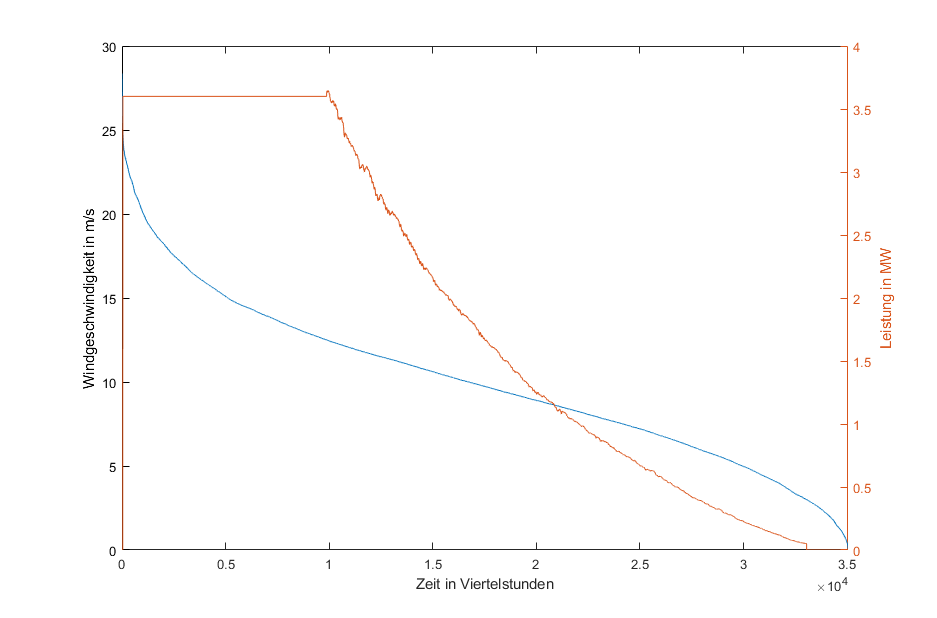
\includegraphics[width=12cm]{img/results/Dauerlinie_Offshore}
		\caption{Dauerlinie der Windgeschwindigkeit und der erzeugten Leistung, für den Standort Butendiek.}
	\end{figure}
	\begin{figure}[H]
		\centering
		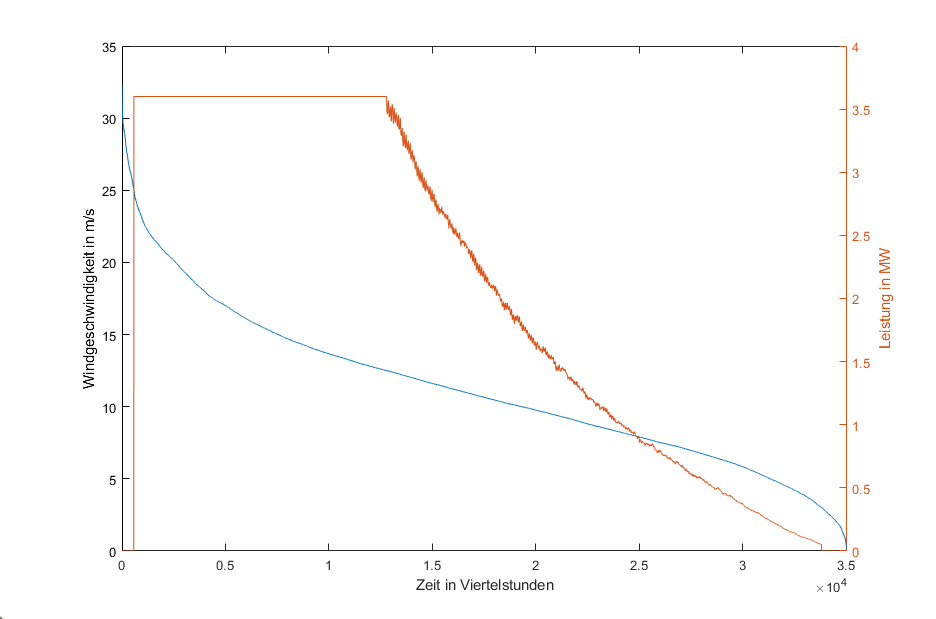
\includegraphics[width=12cm]{img/results/Dauerlinie_Onshore}
		\caption{Dauerlinie der Windgeschwindigkeit und der erzeugten Leistung, für den Standort Joldelund.}
	\end{figure}
	\noindent Der Vergleich von Abbildung 1 und 2 zeigt deutlich, dass die betrachtete Windenergieanlage (SWT-3.6-120) für den Offshore Betrieb konzipiert wurde. Die Anlaufgeschwindigkeit und die Abschaltgeschwindigkeit wurden so parametrisiert, dass sich die Anlage im Offshore Betrieb nur eine geringe Zeit im Flautenbereich und so gut wie nie im abgeschalteten Zustand befindet.\\ \par
	\noindent Der Ertrag kann nun entsprechend Formel 6 errechnet werden.
	\begin{table}[h]
		\centering
		\begin{tabular}{|c|c|c|}
			\hline
			& Butendiek & Joldelund \\ \hline
			Ertrag (in GWh)        & 16.441    & 18.021    \\ \hline
			Volllaststunden (in h) & 4566.9    & 5005.8    \\ \hline
		\end{tabular}
	\end{table}
	\subsection{Betriebskosten und Investitionskosten}
	Die Errichtung von Offshore-Windenergieanlagen bringt signifikat höhere technische und finanzielle Aufwände für die Planung, Errichtung, den Betrieb und den Rückbau mit sich. Die (in den meisten Fällen) höheren Erträge, Anlagennennleistungen und Einspeisevergütungen tragen jedoch dazu bei, dass Offshore Windenergie wirtschaftlich genutzt wird.\\ \par
	\noindent Ein großer Vorteil von Offshore Windparks ist die Möglichkeit jeweils 50 bis 80 Windenergieanlagen in Einheiten bzw. Clustern zu errichten. 
	\noindent 
	\subsection{Barwert}
	\subsection{Lebensdauer}
	\subsection{Zusammenfassung}
	\newpage
	\section{Standort in Europa}
	\subsection{Ertrag}
	\subsection{Barwert}
	\subsection{Zusammenfassung}
	\newpage
	\listoffigures
	\end{document}